\documentclass[12pt letter]{report}
\input{../template/preamble}
\input{../template/macros}
\input{../template/letterfonts}

\usepackage{tikz}
\usepackage{hyperref}
\hypersetup{
    colorlinks=true,
    linkcolor=blue,
    filecolor=magenta,      
    urlcolor=cyan,
    pdftitle={Overleaf Example},
    pdfpagemode=FullScreen,
    }

\urlstyle{same}
\usetikzlibrary{automata, positioning, arrows}
\tikzset{
->, % makes the edges directed
% >=stealth’, % makes the arrow heads bold
node distance=3cm, % specifies the minimum distance between two nodes. Change if necessary.
every state/.style={thick, fill=gray!10}, % sets the properties for each ’state’ node
initial text=$ $, % sets the text that appears on the start arrow
}
\usepackage{booktabs}
\usepackage{karnaugh-map}
\usepackage{parskip}
\usepackage{graphicx}
\graphicspath{ {assets/} }

\title{\Huge{Homework 2}}
\author{\huge{Madiba Hudson-Quansah}}
\date{}


\begin{document}
\maketitle
\newpage

\qs{}{
  \begin{enumerate}
    \item Write the logical expression that indicates $Y$'s functional behaviour
    \item Design a logic circuit network that realizes $Y$'s functional behaviour
    \item Construct a Karnaugh map
    \item Using the Karnaugh map results, re-write the logical expression from part a above
    \item Re-design the logical circuit network from b above and indicate what elements have been
          eliminated from the original logic circuit network.
    \item Write the SOP and POS forms of the given truth table. For this truth table, which form
          is more efficient and convenient and why
    \item Using universal gates NAND and NOR, draw the circuits that realize the logic for
          the SOP
  \end{enumerate}
}

\sol{
  \begin{enumerate}
  \item $Y = \left( A + B + C \right) \left( A + \overline{B} + C \right) \left( \overline{A} + \overline{B} + C \right)   $
  \item
  \begin{figure}[H]
    \begin{center}
      % \includegraphics[width=0.5\textwidth]{circ1.png}
    \end{center}
  \end{figure}
  \item
  \begin{figure}[H]
  \centering
  \begin{karnaugh-map}[4][2][1][$BC$][$A$]
  \maxterms{0,2,6}
  \autoterms[1]
  \implicant{4}{5}
  \implicant{1}{7}
  \end{karnaugh-map}
  \end{figure}
  \item $Y = A\overline{B} + C$
  \item
  \begin{figure}[H]
    \begin{center}
      % \includegraphics[width=0.5\textwidth]{circ2.png}
    \end{center}
  \end{figure}
  Two OR gates and $\overline{A}$ have been removed

  \item
  \begin{align*}
    \text{SOP} & = \overline{A}\overline{B}C + \overline{A}BC + A\overline{B}\overline{C} + A \overline{B}C + ABC                  \\
    \text{POS} & = Y = \left( A + B + C \right) \left( A + \overline{B} + C \right) \left( \overline{A} + \overline{B} + C \right) \\
  \end{align*}
  The POS is more efficient and convenient as it has less terms and therefore requires less gates to construct.
  \item
  \begin{figure}[H]
    \begin{center}
      % \includegraphics[width=0.5\textwidth]{circ3.png}
    \end{center}
  \end{figure}

  \end{enumerate}
}

\qs{}{
  \begin{enumerate}
    \item
          Using Boolean algebra, show that the following two expressions are equivalent:
          \begin{align*}
            F_1 & = \overline{A}BC + A \overline{B} C + A B\overline{C} + ABC                                               \\
            F_2 & = \left( A + B + C \right) \left( A + B + \overline{C} \right) \left( A + \overline{B} + C \right) \left(
            \overline{A} + B + C \right)                                                                                    \\
          \end{align*}
          These two expressions represent the majority function in sum-of-products and product-of-sums form.
    \item
          Assuming that AND, OR, NAND and NOT gates are available, sketch the combinations that would realize the following:
          \begin{enumerate}
            \item $Y = AB\overline{C} + \overline{A + \overline{ \left( B + C \right) }}$
            \item $Z = B \left( A + \overline{\overline{B} + \overline{C}} \right) + \overline{A + \overline{
                        \left( B + C \right)
                      }} $

          \end{enumerate}
    \item
          For the circuit shown below, determine the relationship between the output Z and the inputs A, B and C.    Construct a truth table for the function
    \item
          Provide a circuit diagram that implements the following Boolean function using four inputs (A, B, C, D):
          \[
            F = \left( A + \overline{B} \right) \left( B + C + \overline{D} \right) \left( A + \overline{B} + \overline{C} \right)
          \]
          That has don't care states $AB\overline{C} \overline{D}$, $A B \overline{C} D$, $A B C D$, $A B C \overline{D}$
          \begin{enumerate}
            \item Implement the function above using only NAND gates.
          \end{enumerate}
  \end{enumerate}
}

\sol{
  \begin{enumerate}
    \item
          \begin{align*}
            F_2 & = \left( A + B + C \right) \left( A + B + \overline{C} \right) \left( A + \overline{B} + C \right) \left(
            \overline{A} + B + C \right)                                                                                     \\
                & = A + B + \overline{C}C \left( A + \overline{B} + C \right) \left(
            \overline{A} + B + C \right)                                                                                     \\
                & = A + A\overline{B} + AC + AB + BC \left(
            \overline{A} + B + C \right)                                                                                     \\
                & = A + AC + BC \left(
            \overline{A} + B + C \right)                                                                                     \\
                & = A \left( \overline{A} + B + C \right) +  AC \left( \overline{A} + B + C \right) + BC \left( \overline{A}
            + B + C\right)                                                                                                   \\
                & = AB + AC + ABC + AC + \overline{A}BC + BC + BC                                                            \\
                & = AB + AC + ABC + \overline{A}BC + BC                                                                      \\
                & = ABC + AB\overline{C} + ABC + A\overline{B}C + ABC + \overline{A}BC + ABC + \overline{A}BC                \\
                & = ABC + AB\overline{C} + A\overline{B}C + \overline{A}BC                                                   \\
            F_1 & =ABC + AB\overline{C} + A\overline{B}C + \overline{A}BC                                                    \\
          \end{align*}
          $\therefore$ $F_1 = F_2$
    \item \begin{enumerate}
            \item
                  \begin{figure}[H]
                    \begin{center}
                      % \includegraphics[width=0.5\textwidth]{circ2a1.png}
                    \end{center}
                  \end{figure}
            \item
                  \begin{figure}[H]
                    \begin{center}
                      % \includegraphics[width=0.5\textwidth]{circ2a2.png}
                    \end{center}
                  \end{figure}
          \end{enumerate}
    \item
          \[
            Z = \overline{\overline{A} B + AC}
          \]
          \begin{table}[H]
            \begin{center}
              \begin{tabular}{|c c c|c|}
                \hline
                $A$ & $B$ & $C$ & $\overline{\overline{A} B + AC}$ \\ [0.5ex]
                \hline
                \hline
                0   & 0   & 0   & 1                                \\
                0   & 0   & 1   & 1                                \\
                0   & 1   & 0   & 0                                \\
                0   & 1   & 1   & 0                                \\
                1   & 0   & 0   & 1                                \\
                1   & 0   & 1   & 0                                \\
                1   & 1   & 0   & 1                                \\
                1   & 1   & 1   & 0                                \\
                \hline
              \end{tabular}
            \end{center}
          \end{table}
    \item
          \begin{figure}[H]
            \begin{center}
              % \includegraphics[width=0.5\textwidth]{circ2d1.png}
            \end{center}
          \end{figure}
          \begin{enumerate}
            \item
                  \begin{figure}[H]
                    \begin{center}
                      % \includegraphics[width=0.5\textwidth]{circ2d2.png}
                    \end{center}
                  \end{figure}
          \end{enumerate}
  \end{enumerate}
}

\qs{}{
  A sequential circuit with two D flip-flops $A$ and $B$, two inputs, $x$ and $y$; and one output $z$ is specified by the following next-state and output equations:
  \begin{align*}
    A \left( t + 1 \right) & = \overline{x} y + xA + yA                        \\
    B \left( t + 1 \right) & = \overline{x} B + xA + \overline{x} \overline{A} \\
    z                      & = A + Bx                                          \\
  \end{align*}
  \begin{enumerate}
    \item Draw the logic diagram of the circuit
    \item Provide the state table for the sequential circuit.
    \item Draw the corresponding state diagram.
    \item Is this circuit a Mealy machine or a Moore Machine? Explain why
  \end{enumerate}
}

\sol{
  \begin{enumerate}
    \item
          \begin{figure}[H]
            \begin{center}
              % \includegraphics[width=0.5\textwidth]{circ3a.png}
            \end{center}
          \end{figure}

    \item
          \begin{table}[H]
            \begin{center}
              \begin{tabular}{*{7}{wc{7mm}}} \toprule
                \multicolumn{2}{c}{Current State} &
                \multicolumn{2}{c}{Input}         &
                \multicolumn{2}{c}{Next State}    &
                \multicolumn{1}{c}{Output}                                            \\

                % \cmidrule(lr){1-2}\cmidrule(lr){3-4}\cmidrule{5-6}\cmidrule{7}        \\
                $A$                               & $B$ & $x$ & $y$ & $A$ & $B$ & $z$ \\
                \midrule
                0                                 & 0   & 0   & 0   & 0   & 1   & 0   \\
                0                                 & 0   & 0   & 1   & 1   & 1   & 0   \\
                0                                 & 0   & 1   & 0   & 0   & 0   & 0   \\
                0                                 & 0   & 1   & 1   & 0   & 0   & 0   \\
                \hline
                0                                 & 1   & 0   & 0   & 0   & 1   & 0   \\
                0                                 & 1   & 0   & 1   & 1   & 1   & 0   \\
                0                                 & 1   & 1   & 0   & 0   & 0   & 1   \\
                0                                 & 1   & 1   & 1   & 0   & 0   & 1   \\
                \hline
                1                                 & 0   & 0   & 0   & 0   & 0   & 1   \\
                1                                 & 0   & 0   & 1   & 1   & 0   & 1   \\
                1                                 & 0   & 1   & 0   & 1   & 1   & 1   \\
                1                                 & 0   & 1   & 1   & 1   & 1   & 1   \\
                \hline
                1                                 & 1   & 0   & 0   & 0   & 1   & 1   \\
                1                                 & 1   & 0   & 1   & 1   & 1   & 1   \\
                1                                 & 1   & 1   & 0   & 1   & 1   & 1   \\
                1                                 & 1   & 1   & 1   & 1   & 1   & 1   \\

                \midrule
                \bottomrule
              \end{tabular}
            \end{center}
          \end{table}
    \item
          \begin{figure}[H]
            \centering
            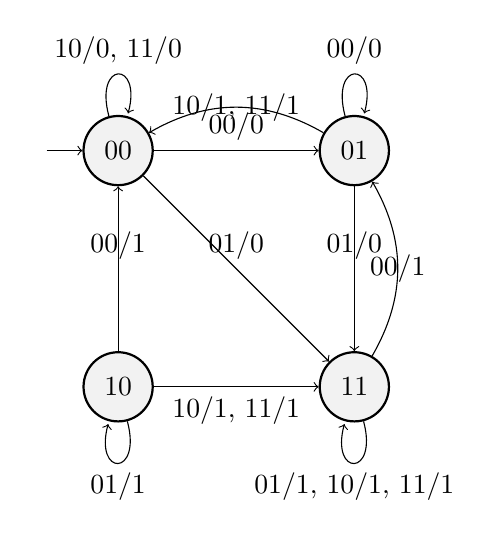
\begin{tikzpicture}
              \node[state, initial] (00) {$00$};
              \node[state,right of=00] (01) {$01$ };
              \node[state, below of=01] (11) {$11$ };
              \node[state, below of=00] (10) {$10$ };

              \draw
              (00) edge[loop above] node{10/0, 11/0} (00)
              (00) edge[above] node{00/0} (01)
              (00) edge[above] node{01/0} (11)

              (01) edge[loop above] node{00/0} (01)
              (01) edge[above] node{01/0} (11)
              (01) edge[bend right] node{10/1, 11/1} (00)

              (11) edge[loop below] node{01/1, 10/1, 11/1} (11)
              (11) edge[bend right] node{00/1} (01)

              (10) edge[loop below] node{01/1} (10)
              (10) edge[above] node{00/1} (00)
              (10) edge[below] node{10/1, 11/1} (11)
              ;
            \end{tikzpicture}
          \end{figure}
    \item
          This is a Mealy machine because the output depends on both the state and input.
  \end{enumerate}
}

\qs{}{
  \begin{enumerate}
    \item Convert each binary number to hexadecimal:
          \begin{enumerate}
            \item 10101010
            \item 10101100
            \item 10111011
          \end{enumerate}
    \item Perform each subtraction in the 2’s complement form:
          \begin{enumerate}
            \item $00110011 - 00010000 $
            \item $01100101 - 11101000$
          \end{enumerate}
    \item Perform the following binary multiplications:
          \begin{enumerate}
            \item $1100 \times 101$
            \item $1110 \times  1110$
          \end{enumerate}
  \end{enumerate}

}

\sol{
  \begin{enumerate}
    \item \begin{enumerate}
            \item $A A$
            \item $A C$
            \item $BB$
          \end{enumerate}
    \item \begin{enumerate}
            \item
                  \begin{align*}
                    \begin{array}{c cccc cccc}
                        & 0 & 0 & 1 & 1 & 0 & 0 & 1 & 1 \\
                      - & 0 & 0 & 0 & 1 & 0 & 0 & 0 & 0 \\
                      \hline
                        & 0 & 0 & 1 & 1 & 0 & 0 & 1 & 1 \\
                      + & 1 & 1 & 1 & 1 & 0 & 0 & 0 & 0 \\
                      \hline
                        & 0 & 0 & 1 & 0 & 0 & 0 & 1 & 1 \\
                    \end{array}
                  \end{align*}
            \item
                  \begin{align*}
                    \begin{array}{c cccc cccc}
                        & 0 & 1 & 1 & 0 & 0 & 1 & 0 & 1 \\
                      - & 1 & 1 & 1 & 0 & 1 & 0 & 0 & 0 \\
                      \hline
                        & 0 & 1 & 1 & 0 & 0 & 1 & 0 & 1 \\
                      + & 0 & 0 & 0 & 1 & 1 & 0 & 0 & 0 \\
                      \hline
                        & 0 & 1 & 1 & 1 & 1 & 1 & 0 & 1 \\
                    \end{array}
                  \end{align*}

          \end{enumerate}
    \item
          \begin{enumerate}
            \item
                  \begin{align*}
                    \begin{array}{c cccccccc}
                             &   &   &   & 1 & 1 & 0 & 0 & \\
                      \times &   &   &   & 0 & 1 & 0 & 1 & \\
                      \hline
                             &   &   &   & 1 & 1 & 0 & 0 & \\
                             &   &   & 0 & 0 & 0 & 0 &   & \\
                             &   & 1 & 1 & 0 & 0 &   &   & \\
                      +      & 0 & 0 & 0 & 0 &   &   &   & \\
                      \hline
                             & 0 & 1 & 1 & 1 & 1 & 0 & 0 & \\
                    \end{array}
                  \end{align*}
            \item
                  \begin{align*}
                    \begin{array}{c cccccccc}
                             &   &   &   & 1 & 1 & 1 & 0 & \\
                      \times &   &   &   & 1 & 1 & 1 & 0 & \\
                      \hline
                             &   &   &   & 0 & 0 & 0 & 0 & \\
                             &   &   & 1 & 1 & 1 & 0 &   & \\
                             &   & 1 & 1 & 1 & 0 &   &   & \\
                      +      & 1 & 1 & 1 & 0 &   &   &   & \\
                      \hline
                      1      & 1 & 0 & 0 & 0 & 1 & 0 & 0 & \\
                    \end{array}
                  \end{align*}
          \end{enumerate}
  \end{enumerate}
}



\end{document}
